\documentclass[conference]{IEEEtran}
\IEEEoverridecommandlockouts
\usepackage[T1]{fontenc}
\usepackage{lmodern}
\usepackage{cite}
\usepackage{amsmath,amssymb}
\usepackage{graphicx}
\usepackage{xcolor}
\usepackage{booktabs}
\usepackage{multirow}
\usepackage{array}
\usepackage{tikz}
\usetikzlibrary{arrows.meta,positioning,shapes.geometric,fit,calc}
\usepackage{pgfplots}
\pgfplotsset{compat=1.16}
\usepackage[hidelinks]{hyperref}
\def\BibTeX{{\rm B\kern-.05em{\sc i\kern-.025em b}\kern-.08em
    T\kern-.1667em\lower.7ex\hbox{E}\kern-.125em X}}

\newcommand{\code}[1]{\texttt{\small #1}}

\begin{document}

\title{Unified Detection of Tenant-Isolation Violations and QoS Fairness Breaches in Multi-Tenant Kubernetes}

\author{
\IEEEauthorblockN{H S Jayanth}
\IEEEauthorblockA{231IT024\\IT418 Cloud Computing}
\and
\IEEEauthorblockN{Suvarna G}
\IEEEauthorblockA{231IT077\\IT418 Cloud Computing}
}

\maketitle

\begin{abstract}
Multi-tenancy, in which many customers share one infrastructure pool, is central to cloud computing, yet Kubernetes runtime detection tools address only half the problem. A shared cluster can fail its tenants in two ways: an \emph{isolation violation} (one tenant improperly reaching another's resources) and a \emph{fairness/QoS violation} (one tenant's workload degrading a co-located tenant, the ``noisy neighbor''). We build a unified runtime detection pipeline covering both: a control-plane monitor (Kubernetes audit log), a network-flow monitor (eBPF via Cilium/Hubble), and a resource monitor (kubelet/cAdvisor), fused by a deterministic correlation layer that declares a fairness violation only when resource pressure coincides with an independently measured victim-side latency breach. We evaluate on a three-tenant kind cluster with eight repeatable injection scenarios, five repetitions each, plus idle and benign-busy negative controls. Fusing control-plane and network-flow signals detects 25 of 25 isolation injections with no false positives, versus recall 0.60 and 0.40 for either alone. For fairness, the victim-side requirement removes the false alarms a pressure-only rule raises on legitimately busy tenants (precision 1.00 vs.\ 0.88 on a fresh validation run) and detects about six times sooner (2.5\,s vs.\ 14.5\,s), at a small recall cost (0.87 vs.\ 0.93). We also report where the result is fragile: it depends on one latency threshold that we selected post hoc and confirmed on independent runs.
\end{abstract}

\begin{IEEEkeywords}
Kubernetes, multi-tenancy, tenant isolation, QoS fairness, noisy neighbor, eBPF, Cilium, runtime detection
\end{IEEEkeywords}

\section{Introduction}
Cloud computing is about sharing. A customer renting compute from a cloud provider does not get a dedicated machine, but a slice of a pool used by many others at the same time. Kubernetes makes this sharing work at scale by grouping workloads into namespaces and enforcing boundaries with RBAC, network policies and resource quotas.

Those boundaries are only as good as their configuration, and they fail in two very different ways. The first is a \emph{security} failure: a misconfigured role binding gives a service account permissions it should not have, or a missing network policy lets traffic flow where it should not. The second is a \emph{performance} failure: one tenant's workload consumes far more CPU or memory than intended, and the tenant running next to it sees slow responses. Nothing unauthorized happened and no security rule was broken, yet a tenant is harmed. This is the classic noisy-neighbor problem, and most security tooling ignores it.

This work builds and quantitatively evaluates a single detection pipeline for both failure modes on a multi-tenant Kubernetes cluster. Our contributions are:
\begin{itemize}
\item a three-source runtime monitoring pipeline (audit log, eBPF network flows, cgroup resource metrics) and a deterministic fusion layer that classifies each anomaly as isolation, fairness, or both;
\item a fairness rule that requires an independent victim-side QoS breach, not just elevated usage, before declaring a violation;
\item eight versioned, idempotent injection scenarios with ground-truth logging, and an evaluation harness with idle \emph{and} benign-busy negative controls;
\item an honest account of what the first evaluation got wrong (a fairness detector that scored zero, scoring artifacts, an over-sensitive threshold) and how each was fixed.
\end{itemize}

\section{Literature Survey}
\subsection{Base paper: DAST for Kubernetes (FSE '25)}
Shamim, Hu and Rahman evaluate three Dynamic Application Security Testing tools against a live Kubernetes deployment and find thousands of CIS-recommended configuration violations that static analysis alone missed~\cite{shamim2025}. Its central argument, that static checks cannot catch violations that only manifest at runtime, directly motivates this project. Its scope is limited, however: it documents findings but builds no detection tool; it considers only security misconfiguration, not resource fairness; it reports no precision, recall, false-positive rate or latency; and it relies on control-plane signals alone, missing violations visible only on the data or resource plane.

\subsection{eBPF-based runtime security}
Falco~\cite{falco} and Cilium/Tetragon provide general-purpose eBPF runtime anomaly detection. Cilium, through Hubble~\cite{hubble}, is the network-layer data source here. These tools treat runtime security generically: none frames detection around cross-tenant boundary violations, and none pairs security detection with a resource-fairness signal.

\subsection{Resource fairness and noisy neighbors}
Work on cloud resource fairness concentrates on scheduling and enforcement (cgroup throttling, Kubernetes QoS classes) rather than on correlating fairness breaches with an independent victim-side performance signal, and it does not connect to tenant-isolation detection.

\subsection{The gap}
We found no IEEE/ACM publication that unifies tenant-isolation security detection and tenant fairness/QoS detection under one fused pipeline evaluated quantitatively across both failure modes.

\section{Motivation}
\textbf{Multi-tenancy is the concern, not a side issue.} A provider's operational question is not ``is this cluster misconfigured?'' but ``are my tenants safely and fairly sharing this pool?'' Existing tooling answers only the security half.

\textbf{The two violation types are invisible to each other's detectors.} A control-plane monitor sees who asked to access what, but is blind to a CPU-hogging batch job that makes no unauthorized API call. An eBPF network monitor sees cross-namespace traffic, but not cgroup throttling, which lives in a different subsystem (kubelet/cAdvisor).

\textbf{Claims need numbers.} Without precision, recall, false-positive rate and detection latency measured against a structured scenario library and a static baseline, claims about detection effectiveness remain anecdotal.

\section{Objectives}
The project has six objectives, built and validated in dependency order: (1) a multi-tenant kind testbed with enforced isolation and a static kube-bench baseline; (2) a control-plane monitor over the Kubernetes audit log; (3) data-plane (Hubble) and resource-plane (kubelet/cAdvisor) monitors; (4) a fusion and classification layer; (5) a CI/CD Trivy image-scan gate; (6) repeatable scenario libraries and a quantitative evaluation harness.

\section{System Design}
\subsection{Architecture}
Fig.~\ref{fig:arch} shows the pipeline. Three independent collectors feed one fusion layer. The data/resource plane is deliberately \emph{two} collectors: Hubble's eBPF probes sit at the network/socket layer and cannot observe cgroup CPU throttling or memory pressure, which live in kubelet/cAdvisor. A k6 load generator supplies the independent victim-side signal.

\begin{figure}[t]
\centering
\resizebox{\columnwidth}{!}{%
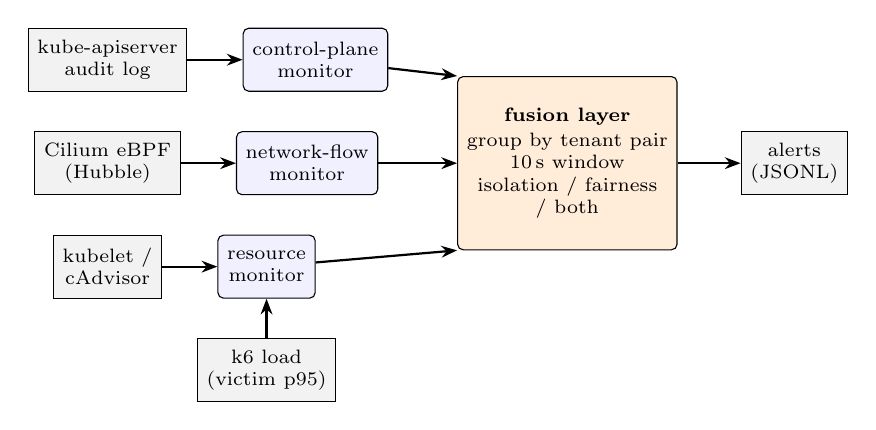
\begin{tikzpicture}[
  node distance=5mm and 7mm,
  box/.style={draw, rounded corners=2pt, align=center, minimum height=8mm, font=\scriptsize, fill=blue!6},
  src/.style={draw, align=center, minimum height=8mm, font=\scriptsize, fill=gray!10},
  fus/.style={draw, rounded corners=2pt, align=center, minimum height=22mm, font=\scriptsize, fill=orange!15},
  arr/.style={-{Stealth[length=2mm]}, thick}]
\node[src] (audit) {kube-apiserver\\audit log};
\node[src, below=of audit] (cil) {Cilium eBPF\\(Hubble)};
\node[src, below=of cil] (kub) {kubelet /\\cAdvisor};
\node[box, right=of audit] (cpm) {control-plane\\monitor};
\node[box, right=of cil] (nfm) {network-flow\\monitor};
\node[box, right=of kub] (rm) {resource\\monitor};
\node[src, below=of rm] (k6) {k6 load\\(victim p95)};
\node[fus, right=10mm of nfm] (fusion) {\textbf{fusion layer}\\[1pt]group by tenant pair\\10\,s window\\isolation / fairness\\/ both};
\node[src, right=8mm of fusion] (alerts) {alerts\\(JSONL)};
\draw[arr] (audit) -- (cpm);
\draw[arr] (cil) -- (nfm);
\draw[arr] (kub) -- (rm);
\draw[arr] (k6) -- (rm);
\draw[arr] (cpm) -- (fusion.north west);
\draw[arr] (nfm) -- (fusion);
\draw[arr] (rm) -- (fusion.south west);
\draw[arr] (fusion) -- (alerts);
\end{tikzpicture}}
\caption{System architecture: three monitors plus a victim-side QoS signal feed one fusion layer.}
\label{fig:arch}
\end{figure}

\subsection{Monitors}
The \textbf{control-plane monitor} tails the API-server audit log (Metadata level) and emits an event when a principal from one tenant's namespace acts on a resource scoped to another. The \textbf{network-flow monitor} wraps \code{hubble observe} and emits events for flows crossing tenant boundaries, including policy-denied egress whose peer identity Hubble does not resolve. The \textbf{resource monitor} polls kubelet/cAdvisor every 10\,s and emits pressure events when a pod's CPU or memory usage reaches 85\% of its limit or it is CFS-throttled. A \textbf{QoS monitor} tails k6 output, freezes a baseline p95 of \code{http\_req\_duration} over the first 10\,s, and emits a \code{victim-qos-latency} breach event whenever the rolling 10\,s p95 reaches a configurable multiple of that baseline (re-emitting every 5\,s while the breach persists).

\subsection{Fusion and classification}
The fusion layer is rule-based and deterministic, which keeps results easy to validate end to end. Events are clustered per tenant pair using a 10\,s sliding window.
\begin{enumerate}
\item \textbf{Isolation:} any cross-namespace control-plane or network-flow event is sufficient evidence on its own.
\item \textbf{Fairness:} resource pressure in one tenant's namespace \emph{and} a victim-side QoS breach in a different tenant, overlapping in time. Elevated usage alone is never enough.
\item \textbf{Both:} an isolation and a fairness cluster for the same tenant pair that overlap in time are merged.
\end{enumerate}
Each alert records the onset of its isolation evidence and of its fairness evidence separately, so that a merged alert can be scored per track (Section~\ref{sec:fixes}).

\subsection{CI/CD gate}
A GitHub Actions workflow builds the demo image and fails the check on any HIGH or CRITICAL vulnerability with a known fix, using Trivy~\cite{trivy}. It is a static, pre-deploy complement to the runtime tracks.

\section{Testbed and Static Baseline}
\subsection{Testbed}
A local kind cluster~\cite{k8s} (one control plane, two workers) runs Cilium~\cite{cilium} in place of the default CNI with Hubble enabled, and API-server audit logging wired to a host-readable file. A FastAPI demo application is deployed once per tenant namespace (\code{tenant-a}, \code{tenant-b}, \code{tenant-c}), each provisioned with a ServiceAccount and read-only Role/RoleBinding scoped to its own namespace; a default-deny Ingress/Egress NetworkPolicy with explicit same-namespace and DNS allows; and a ResourceQuota (\code{limits.cpu: 2}, \code{limits.memory: 1Gi}, \code{pods: 10}) with a LimitRange. These boundaries were verified before any monitor was built on them: a cross-namespace API call is denied, cross-namespace traffic is dropped, and an over-quota pod is rejected.

\subsection{Static baseline: kube-bench}
kube-bench~\cite{kubebench} was run with the CIS 1.9 profile for Kubernetes 1.31 (Table~\ref{tab:kb}). Its weakest area for this project is Policies: 29 WARN, because NetworkPolicy coverage, RBAC scoping and namespace separation are marked Manual. kube-bench can note that a control should be checked but cannot confirm that the specific policies are correct and in force. Since it does not check ResourceQuota or LimitRange at all, a supplementary script confirms both exist for every tenant namespace: all three pass.

\begin{table}[t]
\caption{kube-bench CIS Kubernetes 1.9 results}
\label{tab:kb}
\centering
\begin{tabular}{lrrrr}
\toprule
Category & PASS & FAIL & WARN & INFO\\
\midrule
Master & 40 & 7 & 12 & 0\\
etcd & 7 & 0 & 0 & 0\\
Control Plane & 1 & 0 & 4 & 0\\
Node & 16 & 2 & 6 & 0\\
Policies & 2 & 4 & 29 & 0\\
\midrule
Total & 66 & 13 & 51 & 0\\
\bottomrule
\end{tabular}
\end{table}

\section{Evaluation Methodology}
\subsection{Scenarios}
Eight versioned, idempotent scenarios (each with inject and revert scripts and ground-truth logging) cover both tracks. \emph{Isolation:} NetworkPolicy misconfiguration, RBAC over-permission, credential misuse, privilege escalation, and a data-plane-only crossing (traffic with no API-server footprint). \emph{Fairness:} a CPU-hog batch job, memory pressure, and a ResourceQuota bypass. Each runs five times (25 isolation and 15 fairness runs). All fairness hogs run in \code{tenant-a}, on the node hosting the victim \code{tenant-b}.

\subsection{Controls}
False-positive rate is ill-posed without explicit no-injection windows. We use ten: five \emph{idle} windows, and five \emph{benign-busy} windows in which a well-behaved tenant saturates its own 200m CPU limit with a single small job. Idle windows cannot separate a naive pressure-only rule from the fused rule (neither fires on silence); benign-busy windows can.

\subsection{Detector configurations}
Because configurations differ only in how the same logs are classified, each scenario runs once and is re-scored under every configuration. Isolation: \emph{control-plane-only}, \emph{network-flow-only}, \emph{fused-isolation}. Fairness: \emph{pressure-only} (elevated usage alone is sufficient: the naive baseline) and \emph{fused-fairness} (requires the victim-side breach).

\subsection{Metrics}
An alert matches a run if it is of the right track, involves at least two expected tenants (one for fairness), and its evidence for that track begins within the injection window plus the 10\,s correlation slack. Precision and false-positive rate are computed against the negative-control windows; recall against the injections; detection latency is injection start to the first matching evidence.

\subsection{Creating real contention}
\label{sec:contention}
On our 16-core host, hogs limited to 200m--1.5 cores did not measurably affect a co-located \code{/healthz} handler: victim p95 stayed near 3.6\,ms before and during every injection, so there was no noisy-neighbor effect to detect. We therefore pin the worker node to a 2-CPU cpuset, schedule hogs on the victim's node, and scale them (six 200m CPU hogs; six memory-ramping pods that keep rewriting their working set; a multi-process hog under a 1200m limit for quota bypass). This is engineered contention: per-container CPU limits protected co-located tenants well on a large host.

\section{Results}
\subsection{Main sweep}
Table~\ref{tab:main} gives the sweep: 8 scenarios $\times$ 5 repetitions plus ten controls, with the victim breach ratio at 1.5$\times$.

\begin{table}[t]
\caption{Detector configurations over the full sweep (FP shown as idle/busy windows). The 1.5$\times$ fused-fairness row is the initial threshold; see Table~\ref{tab:thr}.}
\label{tab:main}
\centering
\setlength{\tabcolsep}{3pt}
\begin{tabular}{llrrcccr}
\toprule
Config & Track & TP & FN & FP & Prec. & Recall & Lat.\,(s)\\
\midrule
control-plane-only & iso. & 15 & 10 & 0/0 & 1.00 & 0.60 & 0.22\\
network-flow-only & iso. & 10 & 15 & 0/0 & 1.00 & 0.40 & 0.70\\
\textbf{fused-isolation} & iso. & 25 & 0 & 0/0 & 1.00 & \textbf{1.00} & 0.41\\
\midrule
pressure-only & fair. & 15 & 0 & 0/3 & 0.83 & 1.00 & 13.45\\
fused-fairness (1.5$\times$) & fair. & 13 & 2 & 0/5 & 0.72 & 0.87 & 2.48\\
\bottomrule
\end{tabular}
\end{table}

\textbf{Isolation: the two signals are complementary.} Control-plane-only misses every run of NetworkPolicy misconfiguration and data-plane-only crossing (there is no API call to observe). Network-flow-only misses every run of RBAC over-permission, credential misuse and privilege escalation (no cross-tenant data-plane flow). Fusing them reaches 25/25 with no false positives. A static baseline sees none of these runtime events.

\textbf{Fairness at 1.5$\times$ is worse than the naive rule on precision.} Benign-busy windows reveal that a single 200m job raises victim p95 to 7--9\,ms against 5\,ms idle (1.5--1.8$\times$), so the fused rule fires on all five. Idle windows alone hid this.

\subsection{Threshold sensitivity and validation}
We replayed the sweep's k6 output through the live detector logic at several breach ratios (Table~\ref{tab:thr}, Fig.~\ref{fig:thr}); the replay reproduces the live 1.5$\times$ outcome. At 2.5$\times$ every false alarm disappears while recall is retained. Because this selects the operating point on the data it is scored on, we validated it on a \emph{fresh live run} (new injections and controls) with 2.5$\times$ (Table~\ref{tab:val}). Fused fairness then has no false positives where the naive rule has two, and detects about six times sooner, because kubelet/cAdvisor-derived pressure events arrive tens of seconds after a hog starts whereas the k6 signal is near real time. The price is recall: 0.87 against 0.93, since the fused rule fires only if the victim is actually hurt.

\begin{table}[t]
\caption{Post-hoc replay of fused-fairness at several breach ratios (15 injections; 5 idle, 5 busy controls).}
\label{tab:thr}
\centering
\begin{tabular}{rrrcrr}
\toprule
Ratio & TP & FN & FP idle/busy & Prec. & Lat.\,(s)\\
\midrule
1.5 & 12 & 3 & 0/5 & 0.71 & 2.49\\
1.75 & 15 & 0 & 0/5 & 0.75 & 2.64\\
2.0 & 15 & 0 & 0/4 & 0.79 & 2.77\\
2.5 & 15 & 0 & 0/0 & 1.00 & 4.19\\
3.0 & 15 & 0 & 0/0 & 1.00 & 4.73\\
\bottomrule
\end{tabular}
\end{table}

\begin{figure}[t]
\centering
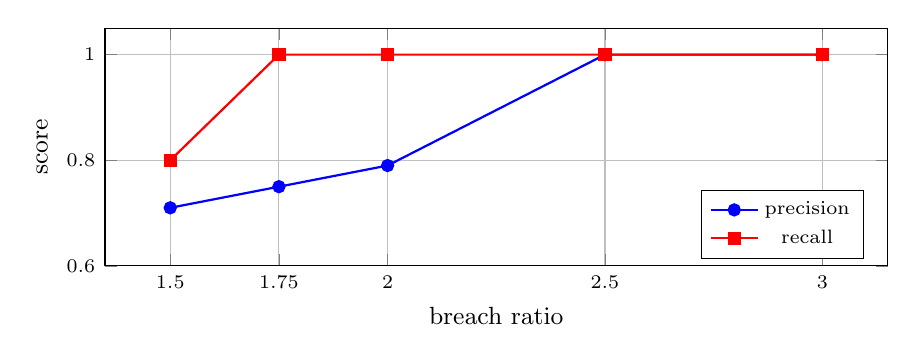
\begin{tikzpicture}
\begin{axis}[width=0.95\columnwidth, height=4.6cm, xlabel={breach ratio}, ylabel={score},
  ymin=0.6, ymax=1.05, xtick={1.5,1.75,2.0,2.5,3.0}, legend pos=south east,
  legend style={font=\scriptsize}, tick label style={font=\scriptsize}, label style={font=\small}, grid=major]
\addplot[blue, mark=*, thick] coordinates {(1.5,0.71)(1.75,0.75)(2.0,0.79)(2.5,1.0)(3.0,1.0)};
\addplot[red, mark=square*, thick] coordinates {(1.5,0.80)(1.75,1.0)(2.0,1.0)(2.5,1.0)(3.0,1.0)};
\legend{precision,recall}
\end{axis}
\end{tikzpicture}
\caption{Fused-fairness precision and recall vs.\ victim breach ratio (post-hoc replay).}
\label{fig:thr}
\end{figure}

\begin{table}[t]
\caption{Fresh validation run at ratio 2.5$\times$ (15 injections; 5 idle, 5 busy controls).}
\label{tab:val}
\centering
\setlength{\tabcolsep}{3pt}
\begin{tabular}{lrrcccr}
\toprule
Config & TP & FN & FP idle/busy & Prec. & Recall & Lat.\,(s)\\
\midrule
pressure-only & 14 & 1 & 0/2 & 0.88 & 0.93 & 14.54\\
\textbf{fused-fairness} & 13 & 2 & 0/0 & \textbf{1.00} & 0.87 & \textbf{2.54}\\
\bottomrule
\end{tabular}
\end{table}

\subsection{Evaluation bugs found and fixed}
\label{sec:fixes}
Our first sweep scored fused fairness at 0 of 15, and later analysis uncovered several problems:
\begin{itemize}
\item \textbf{No victim effect.} The fusion rule was correct, but its required evidence never existed (Section~\ref{sec:contention}). Fixed by the node CPU pin and scaled hogs.
\item \textbf{Edge-triggered QoS events.} One event per breach onset, plus lingering contention between back-to-back runs, produced a single event for a whole sweep. The monitor now re-emits while a breach persists, and the harness waits 45\,s after fairness runs (20\,s otherwise).
\item \textbf{Merged alerts hid detections.} An alert's first-observed time was the earliest evidence of either kind, so lingering fairness evidence merging into an isolation alert pushed its start before the injection window, scoring it a miss (three isolation misses in the second sweep). Alerts now carry per-track onsets; this took fused-isolation from 22/25 to 25/25.
\item \textbf{A meaningless metric.} ``Correlation overhead'' measured the time between an event and scoring, about 330\,s, not fusion cost. It is replaced by measured classifier runtime (about 0.02\,s for 1{,}300 events).
\item \textbf{Flaky tooling.} Version checks using \code{grep -q} under \code{pipefail} intermittently reported tools as missing; fixed.
\end{itemize}

\section{Discussion and Limitations}
\textbf{What the evidence supports.} Signals from different planes catch different violations, so fusion materially improves isolation recall. The fairness rule's value is precision and latency, and it depends on one tunable.

\textbf{Limitations.}
\begin{itemize}
\item \emph{Remaining misses.} In validation, fused fairness missed two of 15 CPU-hog runs: in one the resource monitor never reached its 85\% threshold; in the other an earlier breach merged into the alert so it began before the injection window.
\item \emph{Post-hoc threshold.} The 2.5$\times$ ratio was chosen after seeing data and confirmed on one fresh run, not cross-validated. With 15 runs per condition, intervals are wide.
\item \emph{Engineered contention, single host, one trivial victim workload} (\code{/healthz} through a port-forward). Results may not transfer to production multi-node clusters.
\item \emph{Unaccounted alerts.} Alerts matching no run are reported in the output but not counted as false positives; many are repeat alerts for the same cluster, but we have not audited them, so precision is measured against the control windows only.
\item \emph{Operational dependencies.} The audit log is root-owned on the host, requiring a workaround for the monitor to read it.
\item \emph{Scope.} Automatic remediation was an accepted stretch goal and is not implemented.
\end{itemize}

\section{Conclusion}
We built a unified runtime detection pipeline for tenant isolation and QoS fairness in Kubernetes and evaluated it on eight scenarios with idle and benign-busy controls. Fusing control-plane and network-flow evidence detects all 25 isolation injections with no false positives, where each alone detects 60\% or 40\%. Requiring a victim-side QoS breach for fairness eliminates false alarms on legitimately busy tenants and cuts detection latency about six times, at a small recall cost, provided the breach threshold is set above the noise of a lightly loaded victim. The negative result on our first run, and the analysis that explained it, are as informative as the headline numbers. Future work includes cross-validated thresholds, multi-node and more realistic victim workloads, auditing unaccounted alerts, and the remediation stretch goal.

\begin{thebibliography}{00}
\bibitem{shamim2025} S. I. Shamim, H. Hu, and A. Rahman, ``Dynamic Application Security Testing for Kubernetes Deployment: An Experience Report from Industry,'' in \emph{Proc. ACM Int. Conf. Foundations of Software Engineering (FSE)}, 2025.
\bibitem{cilium} Cilium Authors, \emph{Cilium: eBPF-based Networking, Observability, and Security}, 2024. [Online]. Available: https://cilium.io
\bibitem{hubble} Cilium Authors, \emph{Hubble: Network, Service \& Security Observability for Kubernetes}, 2024. [Online]. Available: https://github.com/cilium/hubble
\bibitem{kubebench} Aqua Security, \emph{kube-bench}, 2024. [Online]. Available: https://github.com/aquasecurity/kube-bench
\bibitem{falco} Falco Authors, \emph{Falco: Cloud Native Runtime Security}, 2024. [Online]. Available: https://falco.org
\bibitem{trivy} Aqua Security, \emph{Trivy: Vulnerability Scanner for Containers}, 2024. [Online]. Available: https://github.com/aquasecurity/trivy
\bibitem{k8s} The Kubernetes Authors, \emph{Kubernetes Documentation}, 2024. [Online]. Available: https://kubernetes.io/docs
\end{thebibliography}

\end{document}
